\documentclass[aspectratio=169,11pt]{beamer}

% -----------------------------------------------------------------------
%  Theme
% -----------------------------------------------------------------------
\usetheme{Boadilla}
% No colour theme — all colours set explicitly below

\usepackage{colortbl}

\definecolor{improved}{RGB}{200, 235, 210}
\definecolor{nesblue}{RGB}{0,51,102}
\definecolor{nesgold}{RGB}{163,125,17}
\definecolor{highlight}{RGB}{195,228,240}   % soft steel-blue highlight

% Title page box
\setbeamercolor{title}{fg=white,bg=nesblue}
\setbeamercolor{subtitle}{fg=nesblue!80,bg=white}
\setbeamercolor{author}{fg=nesblue}
\setbeamercolor{institute}{fg=nesblue}
\setbeamercolor{date}{fg=nesblue}

% Frame titles
\setbeamercolor{frametitle}{fg=white,bg=nesblue}
\setbeamercolor{structure}{fg=nesblue}

% Boadilla palette (drives footline background, etc.)
\setbeamercolor{palette primary}{fg=white,bg=nesblue}
\setbeamercolor{palette secondary}{fg=white,bg=nesblue!85}
\setbeamercolor{palette tertiary}{fg=white,bg=nesblue!70}
\setbeamercolor{palette quaternary}{fg=white,bg=nesblue}

% Blocks
\setbeamercolor{block title}{fg=white,bg=nesblue}
\setbeamercolor{block body}{bg=nesblue!8}
\setbeamercolor{block title alerted}{fg=white,bg=nesgold!85}
\setbeamercolor{block body alerted}{bg=nesgold!10}

\setbeamercolor{alerted text}{fg=nesgold}
\setbeamerfont{frametitle}{series=\bfseries}

% Custom footline: left = author, centre = short title, right = X / N
\setbeamertemplate{footline}{%
  \leavevmode%
  \hbox{%
    \begin{beamercolorbox}[wd=.28\paperwidth,ht=2.25ex,dp=1ex,left,
                           leftskip=1em]{author in head/foot}%
      \usebeamerfont{author in head/foot}\insertshortauthor\ (NES)
    \end{beamercolorbox}%
    \begin{beamercolorbox}[wd=.44\paperwidth,ht=2.25ex,dp=1ex,center]{title in head/foot}%
      \usebeamerfont{title in head/foot}\insertshorttitle
    \end{beamercolorbox}%
    \begin{beamercolorbox}[wd=.28\paperwidth,ht=2.25ex,dp=1ex,right,
                           rightskip=1em]{date in head/foot}%
      \usebeamerfont{date in head/foot}%
      \insertframenumber\,/\,\inserttotalframenumber
    \end{beamercolorbox}}%
  \vskip0pt%
}

% -----------------------------------------------------------------------
%  Packages
% -----------------------------------------------------------------------
\usepackage{amsmath,amssymb,bm}
\usepackage{booktabs}
\usepackage{graphicx}
\usepackage[table]{xcolor}
\usepackage{multirow}
\usepackage{array}
% \usepackage[style=authoryear, sorting=nyt, maxcitenames=2]{biblatex}
% \addbibresource{references.bib}
\usepackage[round, authoryear]{natbib}
% -----------------------------------------------------------------------
%  Title information
% -----------------------------------------------------------------------
\title[FITS]{It Just FITS:\\
Towards Interpretable Forecasting of Time Series via Flow Matching}
\author[V.\,Balabaev]{Vladislav Balabaev\\[4pt]
        {\small Advisor: Ivan Stelmakh}}
\institute[NES]{New Economic School}
\date{}

% -----------------------------------------------------------------------
\begin{document}
% -----------------------------------------------------------------------

% ===========================  TITLE  ===================================
\begin{frame}
  \titlepage
\end{frame}

% ===========================  OUTLINE  =================================
% NOTE: compile twice for TOC to populate (standard LaTeX behaviour)
\setcounter{tocdepth}{1}
\begin{frame}{Outline}
  \tableofcontents
\end{frame}

% =======================================================================
\section{Motivation}
% =======================================================================

\begin{frame}{Deep Learning for Time Series: A Nuanced Picture}

\begin{columns}[T]

%% LEFT — univariate: DL not always best
\begin{column}{0.48\textwidth}
  \textbf{Univariate: DL is not always superior}
  \vspace{0.4em}
  \begin{itemize}
    \item Linear models beat complex architectures on
    \textbf{univariate} benchmarks
    \item \textbf{DLinear} (AAAI 2023): \textit{``an embarrassingly
    simple one-layer linear model outperforms all existing
    Transformer-based solutions on all 9 benchmarks, often by a
    large margin''} \citep{zeng2023transformers}
  \end{itemize}
\end{column}

\hfill

%% RIGHT — multivariate: DL wins
\begin{column}{0.48\textwidth}
  \textbf{Multivariate: DL recovers the advantage}
  \vspace{0.4em}
  \begin{itemize}
    \item Classical models (VAR, ARIMA) cannot scale to
    high-dimensional cross-variate dependencies
    \item \textbf{iTransformer} (ICLR 2024 Spotlight): \textbf{state-of-the-art} across
    7 real-world datasets, outperforming both Transformers
    \emph{and} linear baselines \citep{liu2024itransformer}
  \end{itemize}
\end{column}

\end{columns}

\end{frame}

\begin{frame}{Deep Learning for Time Series: A Rapidly Growing Field}

\begin{columns}[T]

\begin{column}{0.48\textwidth}
  \textbf{Explosive growth in publications}
  \vspace{0.4em}
  \begin{itemize}
    \item DL-TSF papers at top-6 AI/ML venues (NeurIPS, ICLR,
    ICML, AAAI, IJCAI, KDD) grew $\approx$\textbf{10$\times$}
    from 2021 to 2024 \citep{kim2025survey}
    \item Field has entered a \textit{``renaissance of
    architectural modeling''} \citep{kim2025survey}
  \end{itemize}
\end{column}

\hfill

\begin{column}{0.48\textwidth}
  \textbf{Architectural diversity across paradigms}
  \vspace{0.4em}
  \begin{itemize}
    \item MLPs, CNNs, RNNs, Transformers, GNNs, diffusion models,
    state-space models \citep{benidis2022deep, lim2021time}
    \item Open benchmarking debate continuously drives better
    models \citep{zeng2023transformers}
  \end{itemize}
\end{column}

\end{columns}
\end{frame}

\begin{frame}{Diffusion Models: State of the Art in Generative Modelling}
  \begin{columns}[T]
    \column{0.56\textwidth}
      \begin{itemize}
        \setlength\itemsep{10pt}
        \item Denoising Diffusion Probabilistic Models (DDPM;
              Ho et al., 2020) achieve state-of-the-art quality
              in image synthesis
        \item \textbf{Key strengths:}
          \begin{itemize}
            \item Principled probabilistic framework
            \item Learns complex, multimodal distributions
            \item Full predictive distribution — not a point estimate
          \end{itemize}
      \end{itemize}
    \column{0.41\textwidth}
      \begin{block}{Core idea}
        \centering
        $x_T\!\sim\!\mathcal{N}(0,I)
         \;\xrightarrow{\;\text{reverse}\;}
         x_0\!\sim\! p_{\mathrm{data}}$
        \vspace{5pt}

        {\footnotesize Iteratively remove noise to recover
        samples from the data distribution.}
      \end{block}
  \end{columns}
\end{frame}

% -----------------------------------------------------------------------
\begin{frame}{Time Series Forecasting: A Natural Application}
  \begin{itemize}
    \setlength\itemsep{9pt}
    \item \textbf{Goal:} given history
          $\mathbf{x}_{-L+1:0}\!\in\!\mathbb{R}^{L\times D}$,
          produce a \textbf{interpretable} \emph{predictive distribution} over the
          forecast horizon
          $\mathbf{x}_{1:H}\!\in\!\mathbb{R}^{H\times D}$

    \item \textbf{Classical methods} (ARIMA, GARCH): rigid distributional
          assumptions, limited expressivity

    \item \textbf{Deep learning} (Transformers, MLP-Mixer): largely
          point-forecast architectures with poor uncertainty quantification

    \item \textbf{Diffusion for TSF:} treat the future block as a
          \emph{conditional generation problem}
          \[
            p_\theta(\mathbf{x}_{1:H}\mid\mathbf{x}_{-L+1:0})
          \]
          — sample entire future trajectories by progressively denoising
          noise variables, conditioned on the observed context
  \end{itemize}
\end{frame}

% =======================================================================
\section{Background}
% =======================================================================

\begin{frame}{Diffusion Models: Formulation}
  \begin{columns}[T]
    \column{0.50\textwidth}
      \textbf{Forward process}:
      \[
        \mathbf{x}_t
          = \sqrt{\bar\alpha_t}\,\mathbf{x}_0
            + \sqrt{1-\bar\alpha_t}\,\boldsymbol{\epsilon},
        \quad
        \boldsymbol{\epsilon}\sim\mathcal{N}(\mathbf{0},\mathbf{I}),
        \quad t=1,\ldots,T
      \]

      \vspace{4pt}
      \textbf{Conditional reverse denoiser}:
      \[
        \hat{\boldsymbol{\epsilon}}
          = \epsilon_\theta(\mathbf{x}_t,\,\mathbf{c},\,t),
        \qquad
        \mathbf{c} = f_\phi(\mathbf{x}_{-L+1:0})
      \]

      \textbf{Training objective:}
      \[
        \mathcal{L}(\theta)
          = \mathbb{E}_{t,\mathbf{x}_0,\boldsymbol{\epsilon}}
            \bigl[\|\boldsymbol{\epsilon}
                  - \epsilon_\theta(\mathbf{x}_t,\mathbf{c},t)\|_2^2\bigr]
      \]

    % \column{0.46\textwidth}
    %   \centering
    %   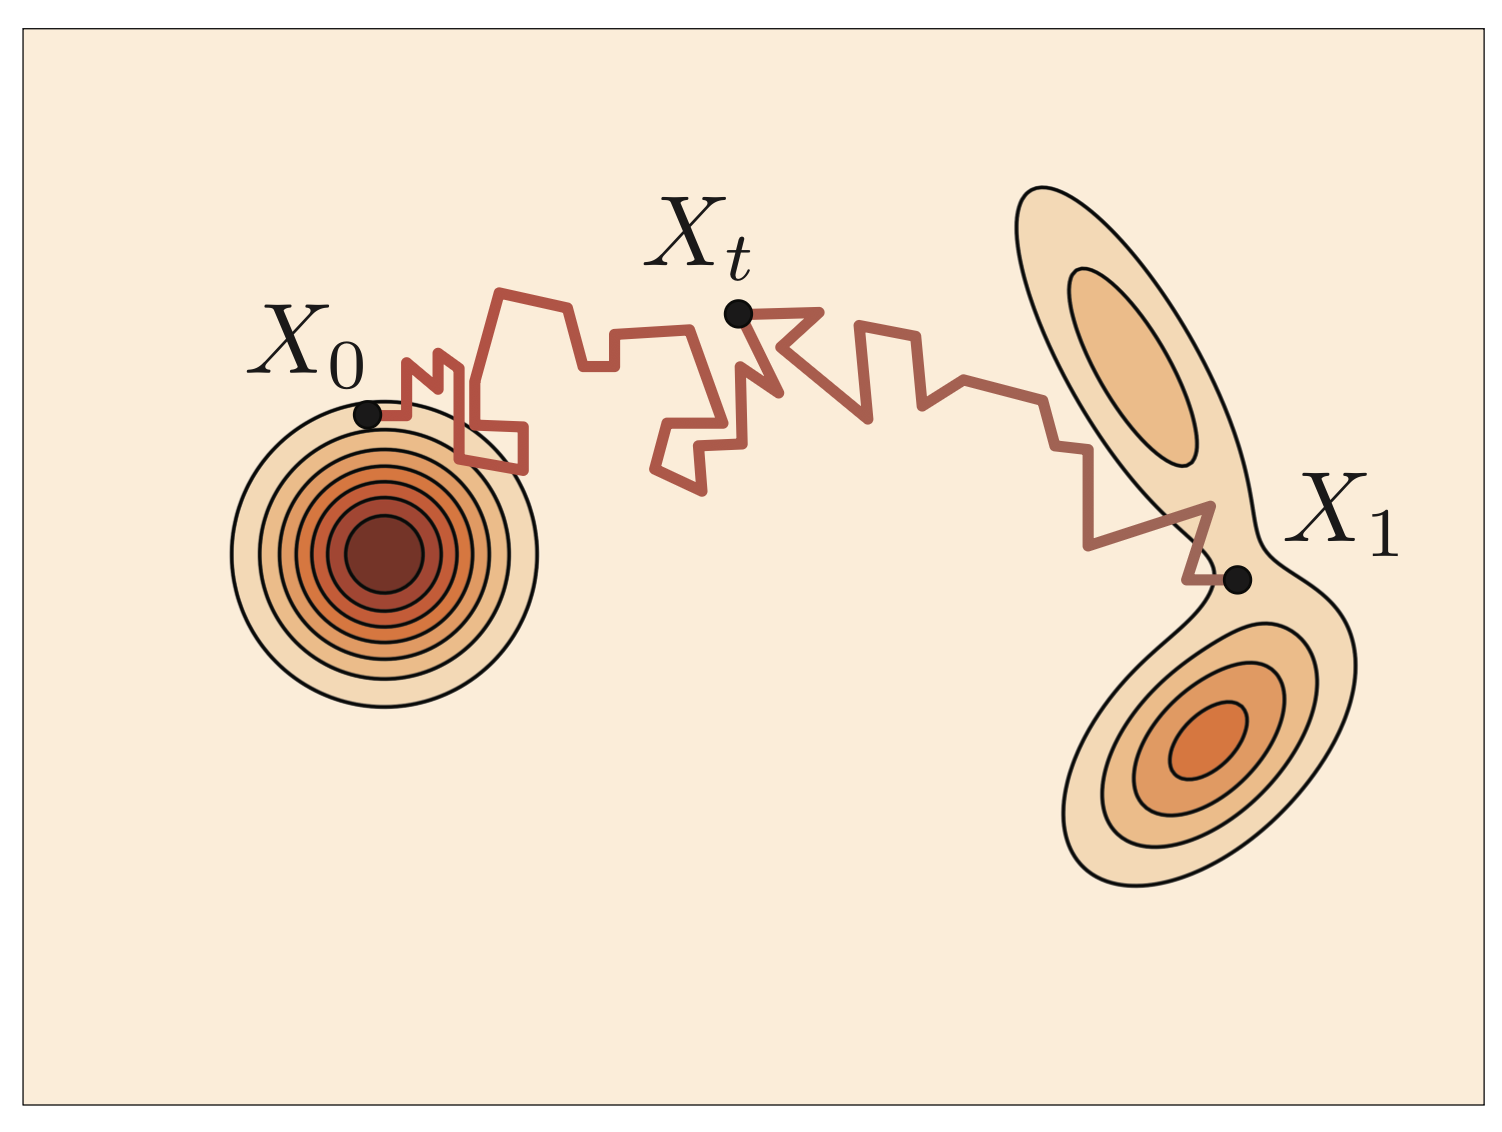
\includegraphics[width=\linewidth,keepaspectratio]{../term_paper/figures/diffusion.png}
  \end{columns}

  \begin{alertblock}{Computational bottleneck}
    Inference requires $\mathcal{O}(10^2\text{--}10^3)$
    denoiser evaluations per forecast sample (Hu et al., 2024).
  \end{alertblock}
\end{frame}

% =======================================================================
\section{Literature Review}
% =======================================================================

\begin{frame}{Key Models in Diffusion-Based TSF}
  \begin{center}
  {\small
  \renewcommand{\arraystretch}{1.0}
  \begin{tabular}{@{}llp{9.5cm}@{}}
    \toprule
    \textbf{Model} & \textbf{Venue} & \textbf{Key design choice} \\
    \midrule
    TimeGrad    & ICML 2021    & RNN encoder; autoregressive diffusion decoding \\
    CSDI        & NeurIPS 2021 & Transformer with joint time–feature self-attention \\
    TimeDiff    & ICML 2023    & Future mixup training; AR initialisation of reverse chain \\
    DiffusionTS & ICLR 2024   & Fourier decomposition; interpretable trend/season heads \\
    mr-Diff     & ICLR 2024   & Multi-resolution seasonal-trend decomposition schedule \\
    LDT         & AAAI 2024   & Latent diffusion; statistics-aware autoencoder (RevIN-like) \\
    S2DBM       & arXiv 2024  & Brownian-bridge diffusion with pinned series endpoints \\
    ARMD        & AAAI 2025   & Future $\!\to\!$ history reversed diffusion trajectory \\
    FALDA       & arXiv 2025  & Fourier-adaptive architecture + dedicated NS-Adapter \\
    NsDiff      & ICML 2025   & Location-Scale Noise Model; uncertainty-aware noise schedule \\
    \bottomrule
  \end{tabular}
  }
  \end{center}
\end{frame}

% -----------------------------------------------------------------------
\begin{frame}{A Comprehensive Survey of the Field}
  \begin{block}{\textit{Diffusion Models for Time Series Forecasting: A Survey}}
    arXiv 2507.14507 \quad (2025)
    \vspace{6pt}
    \begin{itemize}
      \setlength\itemsep{5pt}
      \item Catalogues \textbf{100+} diffusion-based TSF models
            published between 2021 and 2025
      \item Covers standard benchmarks: ETTh, Solar,
            Electricity, Traffic, Weather
      \item Systematically evaluates CRPS, MSE, MAE,
            RMSE across all frameworks
    \end{itemize}
  \end{block}
\end{frame}


\begin{frame}{Field on Non-Stationary Data}
  \begin{block}{}
    \begin{itemize}
      \setlength\itemsep{6pt}
      \item Non-stationarity is addressed in only
            \textbf{3 of 22} well-known models
      \item When addressed, the community overwhelmingly
            prefers decomposition or architectural
            modifications
      \item Classical econometric preprocessing
            (differencing) is entirely absent
    \end{itemize}
  \end{block}
\end{frame}

\section{Contributions}
% =======================================================================

\begin{frame}{Main Contributions}
  \begin{enumerate}
    \setlength\itemsep{14pt}

    \item \textbf{Flow matching for conditional probabilistic forecasting.}\\
          Instantiate a rectified-flow / FM objective on the masked
          forecasting task, achieving inference-time efficiency
          far exceeding standard diffusion.

    \item \textbf{First-difference stationarization.}\\
          Model increments $\Delta\mathbf{x}_t = \mathbf{x}_t - \mathbf{x}_{t-1}$
          instead of levels. Removes drift and time-varying marginal
          moments, yielding a more stable conditional target distribution
          that is substantially easier for any generative model to learn.

    \item \textbf{Jump component via Hawkes-style self-excitation.}\\
          Extend the DiffusionTS decoder with an explicit jump head
          $\mathbf{J}$ — a causally filtered, self-exciting
          signal standard in financial econometrics. Adds both
          \emph{interpretability} and forecast accuracy without
          significant parameter overhead.
  \end{enumerate}
\end{frame}

% =======================================================================
\section{Methodology}
% =======================================================================

% -----------------------------------------------------------------------
\begin{frame}{Flow Matching: A More Efficient Alternative}
  \textbf{Continuous-time ODE} transporting
  $\mathbf{z}_0\!\sim\!\mathcal{N}(0,I)$ to data $\mathbf{z}_1=\mathbf{x}$:
  \[
    \frac{d\mathbf{z}(t)}{dt}
      = \mathbf{v}_\theta(\mathbf{z}(t),\,t,\,\mathbf{c}),
    \qquad
    \mathbf{c} = f_\phi(\mathbf{x}_{-L+1:0})
  \]

  \textbf{Conditional FM loss}
  (straight coupling $\mathbf{z}_t = t\mathbf{z}_1 + (1-t)\mathbf{z}_0$):
  \[
    \mathcal{L}(\theta)
      = \mathbb{E}\bigl[
          \|\mathbf{M}\odot
            (\mathbf{v}_\theta(\mathbf{z}_t,t)
             - (\mathbf{z}_1 - \mathbf{z}_0))\|_2^2
        \bigr]
  \]
  where $\mathbf{M}$ is the forecast mask; observed indices are clamped.

  \vspace{6pt}
  \begin{block}{Rectified flow (Liu et al., 2022)}
    Optimises for straight transport trajectories
    $\;\Rightarrow\;$ accurate generation with as few as
    \textbf{1--10 ODE steps} at inference — far cheaper than diffusion.
  \end{block}
\end{frame}

\begin{frame}{FITS: Architecture Overview}
  \vspace{6pt}
  \begin{columns}[T]
    \column{0.52\textwidth}
      \textbf{Encoder} (Transformer):
      \begin{itemize}
        \item Conv-MLP embedding $\to$ self-attention
              with RoPE and RMSNorm
        \item AdaLN diffusion-time conditioning (DiT-style)
      \end{itemize}
      \vspace{6pt}
      \textbf{Decoder} (alternating self- and cross-attention):
      \begin{itemize}
        \item Accumulates decomposition across $L_d$ layers:
          \[
            (\mathbf{T},\mathbf{S},\mathbf{J})
              = \textstyle\sum_\ell
                (\Delta\mathbf{T}_\ell,\Delta\mathbf{S}_\ell,\Delta\mathbf{J}_\ell)
          \]
        \item \textbf{Reconstruction:}
              $\hat{\mathbf{x}} = \mathbf{T}+\mathbf{S}+\mathbf{J}+\mathbf{E}$
      \end{itemize}

    \column{0.45\textwidth}
      \begin{block}{Decomposition heads}
        \begin{itemize}
          \setlength\itemsep{10pt}
          \item $\mathbf{T}$: degree-3 polynomial basis (N-BEATS)
          \item $\mathbf{S}$: inverse-DFT Fourier reconstruction
                (FEDformer)
          \item $\mathbf{J}$: Hawkes-style excitation
          \item $\mathbf{E}$: residual via inverse projection
        \end{itemize}
      \end{block}
  \end{columns}
\end{frame}


% =======================================================================
\section{Empirical Results}
% =======================================================================

\begin{frame}{Quantitative Results — First Differences}
\begin{table}[ht]
\centering
\caption{Comparison of forecasting performance without $\rightarrow$ with first differeces.}
\label{tab:fd_comparison}
\resizebox{\textwidth}{!}{
\begin{tabular}{l ccc ccc}
\toprule
& \multicolumn{3}{c}{\textbf{MAE} $\downarrow$} & \multicolumn{3}{c}{\textbf{CRPS} $\downarrow$} \\
\cmidrule(lr){2-4} \cmidrule(lr){5-7}
\textbf{Model} & Electricity & ETTh & Exchange & Electricity & ETTh & Exchange \\
\midrule
iTransformer  & \cellcolor{improved!40} 32.937 $\rightarrow$ 26.204 & \cellcolor{improved!40} 1.418 $\rightarrow$ 1.411 & \cellcolor{improved!40} 0.010 $\rightarrow$ 0.010 & \cellcolor{improved!40} 0.108 $\rightarrow$ 0.086 & \cellcolor{improved!40} 0.269 $\rightarrow$ 0.268 & \cellcolor{improved!40} 0.014 $\rightarrow$ 0.014 \\
Diffusion-TS  & 42.137 $\rightarrow$ 43.626 & 2.355 $\rightarrow$ 2.472 & 0.010 $\rightarrow$ 0.038 & 0.113 $\rightarrow$ 0.125 & \cellcolor{improved!40} 0.398 $\rightarrow$ 0.369 & 0.012 $\rightarrow$ 0.053 \\
\textbf{CSDI}          & \cellcolor{improved!40} 29.740 $\rightarrow$ 25.726 & \cellcolor{improved!40} 1.812 $\rightarrow$ 1.515 & 0.010 $\rightarrow$ 0.011 & \cellcolor{improved!40} 0.074 $\rightarrow$ 0.065 & \cellcolor{improved!40} 0.262 $\rightarrow$ 0.217 & 0.012 $\rightarrow$ 0.013 \\
PatchTST      & \cellcolor{improved!40} 38.008 $\rightarrow$ 29.398 & \cellcolor{improved!40} 1.587 $\rightarrow$ 1.364 & \cellcolor{improved!40} 0.010 $\rightarrow$ 0.010 & \cellcolor{improved!40} 0.125 $\rightarrow$ 0.097 & \cellcolor{improved!40} 0.301 $\rightarrow$ 0.259 & \cellcolor{improved!40} 0.015 $\rightarrow$ 0.014 \\
TimeGrad      & \cellcolor{improved!40} 45.175 $\rightarrow$ 34.790 & \cellcolor{improved!40} 2.075 $\rightarrow$ 1.870 & 0.010 $\rightarrow$ 0.056 & \cellcolor{improved!40} 0.114 $\rightarrow$ 0.091 & \cellcolor{improved!40} 0.313 $\rightarrow$ 0.276 & 0.011 $\rightarrow$ 0.067 \\
\midrule
MrDiff        & \cellcolor{improved!40} 54.307 $\rightarrow$ 39.863 & \cellcolor{improved!40} 2.168 $\rightarrow$ 1.751 & 0.010 $\rightarrow$ 0.021 & \cellcolor{improved!40} 0.178 $\rightarrow$ 0.131 & \cellcolor{improved!40} 0.411 $\rightarrow$ 0.332 & 0.014 $\rightarrow$ 0.031 \\
NSDiff        & \cellcolor{improved!40} 139.337 $\rightarrow$ 46.537 & \cellcolor{improved!40} 4.768 $\rightarrow$ 2.254 & \cellcolor{improved!40} 0.215 $\rightarrow$ 0.040 & \cellcolor{improved!40} 0.340 $\rightarrow$ 0.121 & \cellcolor{improved!40} 0.672 $\rightarrow$ 0.318 & \cellcolor{improved!40} 0.222 $\rightarrow$ 0.044 \\
FALDA         & \cellcolor{improved!40} 42.796 $\rightarrow$ 33.641 & \cellcolor{improved!40} 25.559 $\rightarrow$ 2.416 & \cellcolor{improved!40} 0.312 $\rightarrow$ 0.067 & \cellcolor{improved!40} 0.111 $\rightarrow$ 0.089 & \cellcolor{improved!40} 4.652 $\rightarrow$ 0.373 & \cellcolor{improved!40} 0.428 $\rightarrow$ 0.088 \\
\bottomrule
\end{tabular}
}
\end{table}
\end{frame}

\begin{frame}{Quantitative Results — FITS}
\begin{table}[ht]
\centering
\caption{...}
\label{tab:csdi_fd}
\resizebox{\textwidth}{!}{
\begin{tabular}{l ccc ccc}
\toprule
& \multicolumn{3}{c}{\textbf{MAE} $\downarrow$} & \multicolumn{3}{c}{\textbf{CRPS} $\downarrow$} \\
\cmidrule(lr){2-4} \cmidrule(lr){5-7}
\textbf{Model} & Electricity & ETTh & Exchange & Electricity & ETTh & Exchange \\
\midrule
CSDI    & 29.740 & 1.812 & 0.010 & 0.074 & 0.262 & 0.012 \\
$\Delta$CSDI & 25.726 & 1.515 & 0.011 & 0.065 & 0.217 & 0.013 \\
\midrule
FITS & 30.213 & 1.814 & 0.011 & 0.074 & 0.283 & 0.012 \\
FITS+J & 29.515 & 1.744 & 0.012 & 0.076 & 0.260 & 0.012 \\
$\Delta$FITS & 26.010 & 1.537 & 0.011 & 0.068 & 0.242 & 0.012 \\
$\Delta$FITS+J & 24.212 & 1.499 & 0.009 & 0.060 & 0.225 & 0.011 \\
\bottomrule
\end{tabular}
}
\end{table}
\end{frame}

% -----------------------------------------------------------------------
% \begin{frame}{Qualitative Results — FITS on Electricity Dataset}
%   \centering
%   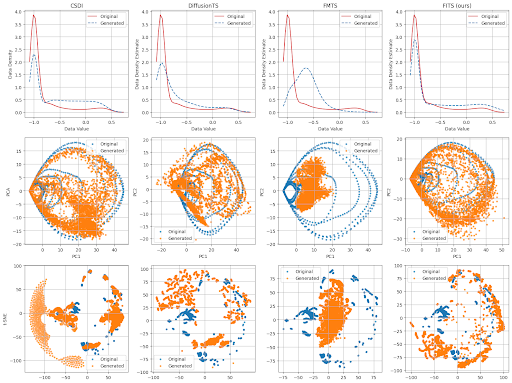
\includegraphics[height=0.78\textheight,keepaspectratio]{../term_paper/figures/dist_solar.png}\\[3pt]
%   {\small Forecast distribution on Electricity}
% \end{frame}

% \begin{frame}{Qualitative Results — Electricity Dataset}
%   \centering
%   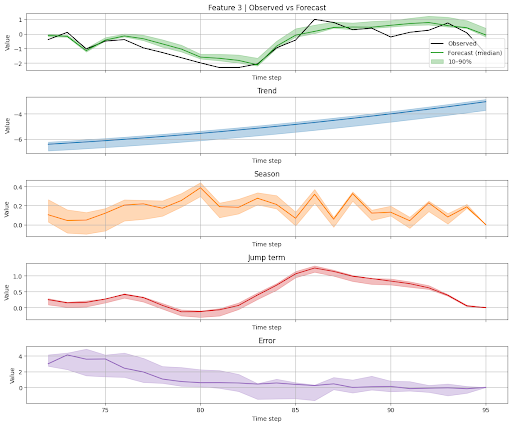
\includegraphics[height=0.78\textheight,keepaspectratio]{../term_paper/figures/interpret_solar.png}\\[3pt]
%   {\small Component decomposition (T\,/\,S\,/\,J\,/\,E) on Electricity}
% \end{frame}

% =======================================================================
\section{Conclusion}
% =======================================================================

\begin{frame}{Conclusion}
  \begin{itemize}
    \setlength\itemsep{10pt}

    \item \textbf{First differencing is underexplored.}\\
          A simple, theoretically motivated, zero-parameter transformation
          that renders the conditional target distribution stationary and
          consistently improves all models that adopt it — without any
          other architectural modification.

    \item \textbf{The gap from the literature is genuine.}\\
          Zero of 30+ diffusion-based TSF models apply first differencing.
          Even ARMD — explicitly ARMA-inspired — omits it.

    \item \textbf{FITS achieves state-of-the-art results on Solar.}\\
          Best on RMSE, MAE, and CRPS$_\Sigma$, with full interpretable
          decomposition into trend, seasonality, jump, and residual
          retrieved at inference time.

  \end{itemize}
\end{frame}

% -----------------------------------------------------------------------
\begin{frame}[plain]
  \centering
  \vspace{1.8cm}
  {\Large\color{nesblue} Thank you for your attention.}\\[14pt]
  {\normalsize Questions are welcome.}\\[22pt]
  \rule{0.5\textwidth}{0.4pt}\\[10pt]
  {\small
    Vladislav Balabaev \quad\textbar\quad New Economic School\\[3pt]
    Advisor: Ivan Stelmakh
  }
\end{frame}

% \begin{frame}[allowframebreaks]{References}
%   \printbibliography
% \end{frame}

\bibliographystyle{plainnat}
\bibliography{references}


\end{document}
